
\documentclass[a4paper, 10pt]{article}
\usepackage[english]{babel}
\usepackage[T1]{fontenc}
\usepackage[utf8]{inputenc}
\usepackage{textcomp}
\setlength{\marginparwidth}{2cm}
\usepackage{comment}
\usepackage{todonotes}
\usepackage{amsmath}
\usepackage{amssymb}
\usepackage{xcolor}
\usepackage{graphicx}
\graphicspath{ {./img/} }
\usepackage{hyperref}
\usepackage{listings}
\usepackage{color}
\definecolor{dkgreen}{rgb}{0,0.6,0}
\definecolor{gray}{rgb}{0.5,0.5,0.5}
\definecolor{mauve}{rgb}{0.58,0,0.82}
\lstset{frame=tb,
  language=Python,
  aboveskip=3mm,
  belowskip=3mm,
  showstringspaces=false,
  columns=flexible,
  basicstyle={\small\ttfamily},
  numbers=none,
  numberstyle=\tiny\color{gray},
  keywordstyle=\color{blue},
  commentstyle=\color{dkgreen},
  stringstyle=\color{mauve},
  breaklines=true,
  breakatwhitespace=true,
  tabsize=3
}
\title{Homework Assignment N°2}
\author{BML36\\Thibault Douzon\\Rajavarman Mathivanan}
\date{September 12th, 2018}
\begin{document}
\maketitle
\pagebreak
\tableofcontents
\pagebreak
\section{Exercise 1: Perceptron Learning Rule}
\subsection{Part a} 
To have an idea of what our perceptron looks like, let's plot its discriminant line 
and the two data points. 
\\ 
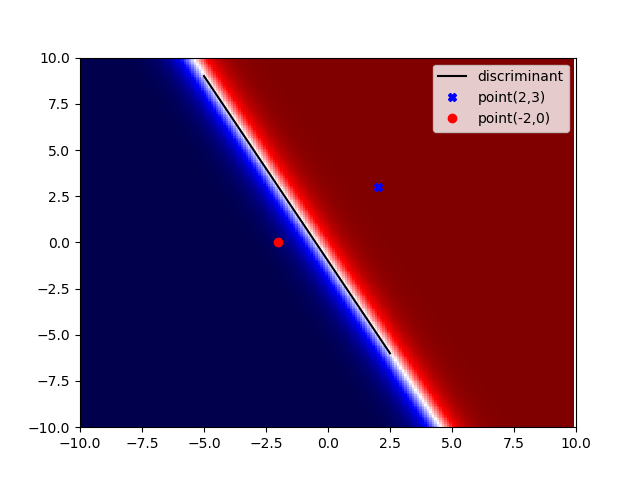
\includegraphics[scale=0.6]{ex1_a.png} 
\\ 
We can also compute the prediction of the model for the two datapoints: 
$$ 
\text{prediction}_1 = sign(w^\top x_1) = sign(8) = 1 \ne -1 
$$ 
$$ 
\text{prediction}_2 = sign(w^\top x_2) = sign(-3) = -1 \ne 1 
$$ 
So our two datapoints are missclassified, now we can say that on the plot below 
area in red (upper right of the plot) represents the area classified as class $1$ by our model and 
blue (lower left part of the plot) is for class $-1$ 
\subsection{Part b} 
After one iteration of a batch learning algorithm we get the following new discriminant: 
$$ 
w_{new} = w_{old} + \eta\sum_{i=1}^N x_ic_i 
$$ 
$$ 
w_{new} = \begin{bmatrix}1 & 0 & -0.5\end{bmatrix} 
$$ 
And now, both data points are acorrectly classified by the new model: 
\\ 
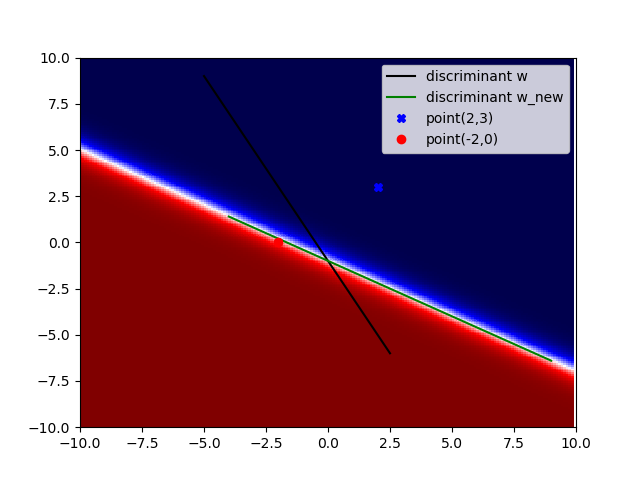
\includegraphics[scale=0.6]{ex1_b.png} 
\subsection{Part c} 
Learning is an iterative process. In a batch version learning, at each iteration we compute a new model 
based on the whole dataset whereas in a stochastic version, at each iteration we pick up a single data in the dataset 
and we base our computation on this data point only. 
\\ 
When the dataset becomes too big, the computation time of a batch iteration is going to need ressources 
proportional to the size of the dataset and a stochastic iteration will always use the same amount of ressources 
independantly of the size of the dataset. 
\subsection{Part d} 
The formula to compute the new discriminant with a stochastic algorithm is the following:
$$
w_{new} = w_{old}+\eta x_i c_i
$$
We repeat it for each data in the dataeset, updating the discriminant at each iteration.
\\
When applying the stochastic algorithm, we get the following (different) result: 
$$ 
w_{new} = \begin{bmatrix}1 & -0.4 & -0.8\end{bmatrix} 
$$ 
And again, both points are correctly classified after the complete sweep: 
\\ 
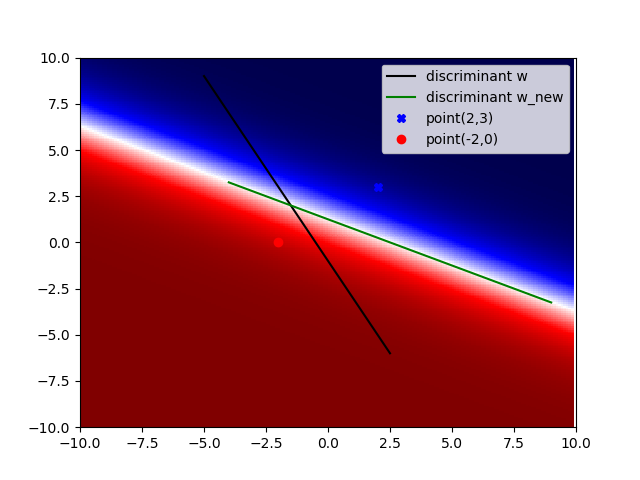
\includegraphics[scale=0.6]{ex1_d.png} 

\section{Exercise 2: Logistic classification \& discrimination}
From now we will use $\sigma(x)=\frac{1}{1+e^{-x}}$
\subsection{Part a}
\begin{itemize}
    \item Initialize $w_0$ ?
    \begin{enumerate}
        \item Some fixed $w_0$ like $\begin{bmatrix}0 & 0 & \cdots & 1\end{bmatrix}$
        \item The result of computation around the dataset like the \\mean: $w_0 = \frac{1}{N}\sum_{i=1}^N x_i$, 
        concatenated with a constant.
        \item A random vector
    \end{enumerate}
    Any vector except the null vector and the multiples of $\begin{bmatrix}1 & 0 & \cdots &0\end{bmatrix}$ is suitable to initialize $w_0$, 
    \item How to learn: for batch learning use this equation at each step
    $$
    w_{n+1} = w_n - \eta \nabla E(w_n) = w_n - \eta \sum_{n=1}^{N}\left(y(n)-t_n\right)x_n
    $$
    \item How to stop the iterative process ?
    \begin{enumerate}
    \item Stop when the norm of the difference vector is low: $\Delta_n = \frac{\left\Vert w_{n+1} - w_n\right\Vert}{\left\Vert w_n \right\Vert} < \epsilon$
    \\
    This is a commonly used criterion that stops the process when the steps we take are getting small compared to our current result.
    \item Stop after fixed number of iteration
    \\
    This ensures we won't enter in a infinite non-convergent process. 
    \item Stop when a threshold error is reached: $E(w_n) < \epsilon $
    \\
    This is actually a bad idea because most of the time we can't be certain it is possible to reach such threshold on the error.
    It would result in an infinite process.
    \end{enumerate}
    In a batch version, we can use criteria 1 and 2 together and stop whenever one of 
    the criteria is reached.
    \\
    In a stochastic version, criterium 1 is not applicable because it would stop the learning process whenever a well classified data
    is picked for an iteration.
\end{itemize}

Our algorithm goes as follows:
\begin{enumerate}
    \item Chose $\epsilon$, $N$ and $\eta$ respectivelly for precision, maximum number of iterations and speed convergency.
    \item Set current error $\Delta$ to $+\infty$ and $n$ to $0$
    \item Chose the initial discriminant: $w_{current} = \begin{bmatrix}0 & 0 & \cdots & 1\end{bmatrix}$.
    \item While $\Delta > \epsilon \wedge n < N$ do
    \begin{enumerate}
        \item Compute and store next discriminant $w_{next}$:
$$
w_{next} = w_{current} - \eta \sum_{n=1}^{N}\left(\sigma({w_{current}}^\top x_n)-t_n\right)x_n
$$
        \item Compute and store the new error $\Delta$:
$$
\Delta = \frac{\left\Vert w_{next} - w_{current}\right\Vert}{\left\Vert w_{current} \right\Vert}
$$
        \item Prepare for next iteration: store $w_{next}$ in place of $w_{current}$ and increment $n$
    \end{enumerate}
    \item If $\Delta > \epsilon$, it means we have not converged enough towards the limit. We should consider increasing N OR using another algorithm for convergence (eg. Newton-Raphson)
    \item Result is stored in $w_{current}$, number of steps in $n$. 
\end{enumerate}

\subsection{Part b}
First important thing to notice is that the point $x=\begin{bmatrix}-1 & 1\end{bmatrix}$ is missclassified.
We define $\bar{x} = \begin{bmatrix}1 & -1 & 1\end{bmatrix}$ thus it means that when we compute 
$w^\top \bar{x}$ the sign of the result is incorrect.
\\
In our case, $w^\top \bar{x} = 1 >0$, thus the real class of $x$ is $0$.
\\
The formula to update the weights is the following:
$$
w_{new} = w - \eta (\sigma(w^\top \bar{x})-t)\bar{x}
$$
We get the following result:
$$
w_{new} \approx \begin{bmatrix}0.5614 & 2.4386 & 1.5614\end{bmatrix}
$$


\section{Exercise 3: Error function \& Gradient descent}
\subsection{Part a}
If $y_n = \sigma(w^\top x_n)$ then:
$$
E(w) = \sum_{n=1}^N (t_n-y_n)^4
$$
$$
\nabla_w E(w) = -4\sum_{n=1}^N (t_n-y_n)^3(y_n (1-y_n))x_n
$$

\subsection{Part b}
$$
E(w) = \sum_{n=1}^N \vert t_n - y_n \vert
$$
Computing the gradient of an absolute value implies to derivate an
absolute value function which  is not $C^1$. We won't be able to assign 
a value to the gradient if the value inside the absolute function is 0.
$$
\nabla_w E(w) = \sum_{n=1}^N y_n(1-y_n)x_n \times \left\{ \begin{array}{ll}  
                    -1 & \text{if $t_n-y_n > 0$}
                \\ 
                    1 & \text{if $t_n-y_n < 0$}
                        \end{array}
                \right.
$$

\section{Exercise 4: MCQ}
\subsection{First MCQ}
This first question tests if the candidate knows how to compute the new
discriminant from the previous one, using gradient descent.
\\
Q: Which of the following equations can be used to update the discriminant $w$ using
the method of gradient descent ?
\\
\begin{enumerate}
    \item $w_{n+1} - w_{n} =  \eta \nabla E(w_{n})$
    \item $w_{n+1} = w_{n} - \eta \nabla E(w_{n})$
    \item $w_{n} + \eta \nabla E(w_{n-1}) = w_{n-1} $
    \item $w_{n} = \eta w_{n} - \nabla E(w_{n+1})$
\end{enumerate}
\subsection{Second MCQ}
The second question verifies the student understood well what is implied behind 
the omnipresent formula $w^\top x$ and each of its components.
\\
Q: When learning in a $k$-dimensions space, knowing that we compute the class of $x$
by the following formula $C(x) = h(w^\top x + w_0)$ where $h$ is the heaviside function. What are
the ranges of $w$ and $x$ ?
\begin{enumerate}
    \item $\begin{array}{cccc}range(w) = k & & & range(x) = k\end{array}$
    \item $\begin{array}{cc}range(w) = k+1 & range(x) = k\end{array}$
    \item $\begin{array}{cccc}range(w) = k & & & range(x) = k+1\end{array}$
    \item $\begin{array}{cc}range(w) = k+1 & range(x) = k+1\end{array}$
\end{enumerate}
\end{document}
\begin{lstlisting}
    # Some python code
\end{lstlisting}